
\subsection{Overview}
The architecture of the system is composed of two main components: the \ac{eMSP} and the \ac{CPMS}.

\subsubsection{\ac{eMSP} overview}

\begin{figure}[!h]
    \begin{center}
        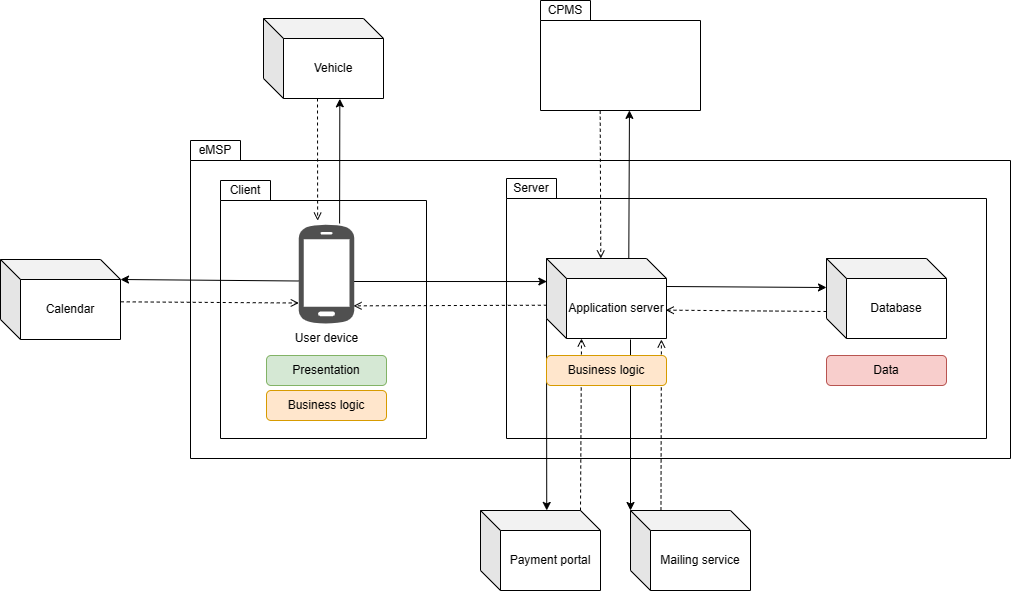
\includegraphics[keepaspectratio, width=0.75\textwidth]{Graphics/DD-eMSP-overview.drawio.png}
        \caption{\ac{eMSP} architectural overview}
        \label{fig:eMSP-overview-architecture}
    \end{center}
\end{figure}

The \ac{eMSP} is a \textbf{three-tier} architecture with \textbf{fat-clients} as seen in \autoref{fig:eMSP-overview-architecture}. This architecture is chosen for different reasons:
\begin{itemize}
    \item Makes the system more scalable;
    \item Allows the separation between business logic and data so that we can apply different levels of dependability to different decoupled systems and we can manage how data is accessed in a more granular way;
    \item There will be a lot of data to be handled in this system (such as booked charges, all the infos about \acp{CPO}, etc.); for this, a dedicated and optimized infrastructure is chosen to be the best choice;
    \item The database will only be accessible by the middleware, constituting an additional layer of security;
    \item With fat-clients the number of messages transmitted are fewer and lighter: an initial elaboration can be done on the smart devices of the user without sending a lot of raw data to the remote application server. The local on-the-edge elaboration is not considered as a problem given the computational power of smartphones.
\end{itemize}
The software pattern applied for this architecture will be the \textbf{\ac{MVC} pattern}. This is the best suit for our application because, being it a web application, we want the components to be as modular, flexible and scalable as possible in order to simplify their distribution.

The following paragraphs will describe the principal components of this pattern and their architectural distribution.

\paragraph{Model}
The model is the logical representation of the persistent data. This is stored in a database system and will only be directly accessible by the server application.

\paragraph{View}
The view logic will be completely delegated to the client application, representing in different ways the data retrieved from the model (e.g. the charging stations sorting based on the user selected preferences).

\paragraph{Controller}
The controller will have to manage all the client requests, interacting with the model, modifying it and returning to the view the changed/retrieved data.
In our application, for the most part, the business logic will be in the server application. Just the part of retrieving and processing the vehicle data the calendar appointments (in the case of a request for smart suggestions of the application) will be handled by the client application so that the communication with the application server will be as simple as possible.

\subsubsection{\ac{CPMS} overview}

\begin{figure}[!h]
    \begin{center}
        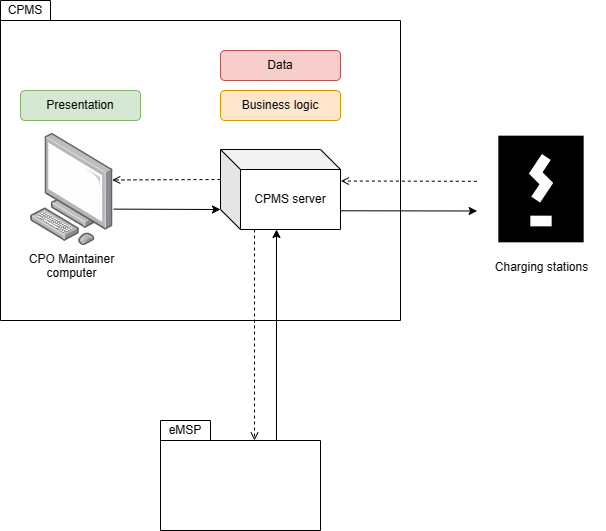
\includegraphics[keepaspectratio, width=0.75\textwidth]{Graphics/DD-CPMS-overview.drawio.png}
        \caption{\ac{CPMS} architectural overview}
        \label{fig:CPMS-overview-architecture}
    \end{center}
\end{figure}

The \ac{CPMS} follows the \textbf{two-tier} pattern with \textbf{thin-clients} as seen in \autoref{fig:CPMS-overview-architecture}. This architecture is chosen for different reasons:
\begin{itemize}
    \item The system is simpler to implement with respect to the three-tier architecture;
    \item The system shouldn't handle so much data, so it isn't necessary to have a dedicated architecture for the data layer;
    \item Clients are thin because they only have to view infos about charging stations and can send simple events (for example \textit{use \ac{DSO} X for charging station Y}, \textit{set revenue percentage to Z}, etc.).
\end{itemize}
Also for this system we will use the \ac{MVC} pattern. In this case, the client will only have the view logic and can send simple events. All the elaboration, the management of the \acp{DSO} and activation/deactivation of charging process of batteries are handled by the \ac{CPMS} server, which handles the business logic and the data.
The \ac{CPMS} server, on the other hand, will deal also with charging requests from \acp{eMSP}, to which it will respond with the elaborated data.


\subsection{Component view}
\begin{figure}[!h]
    \begin{center}
        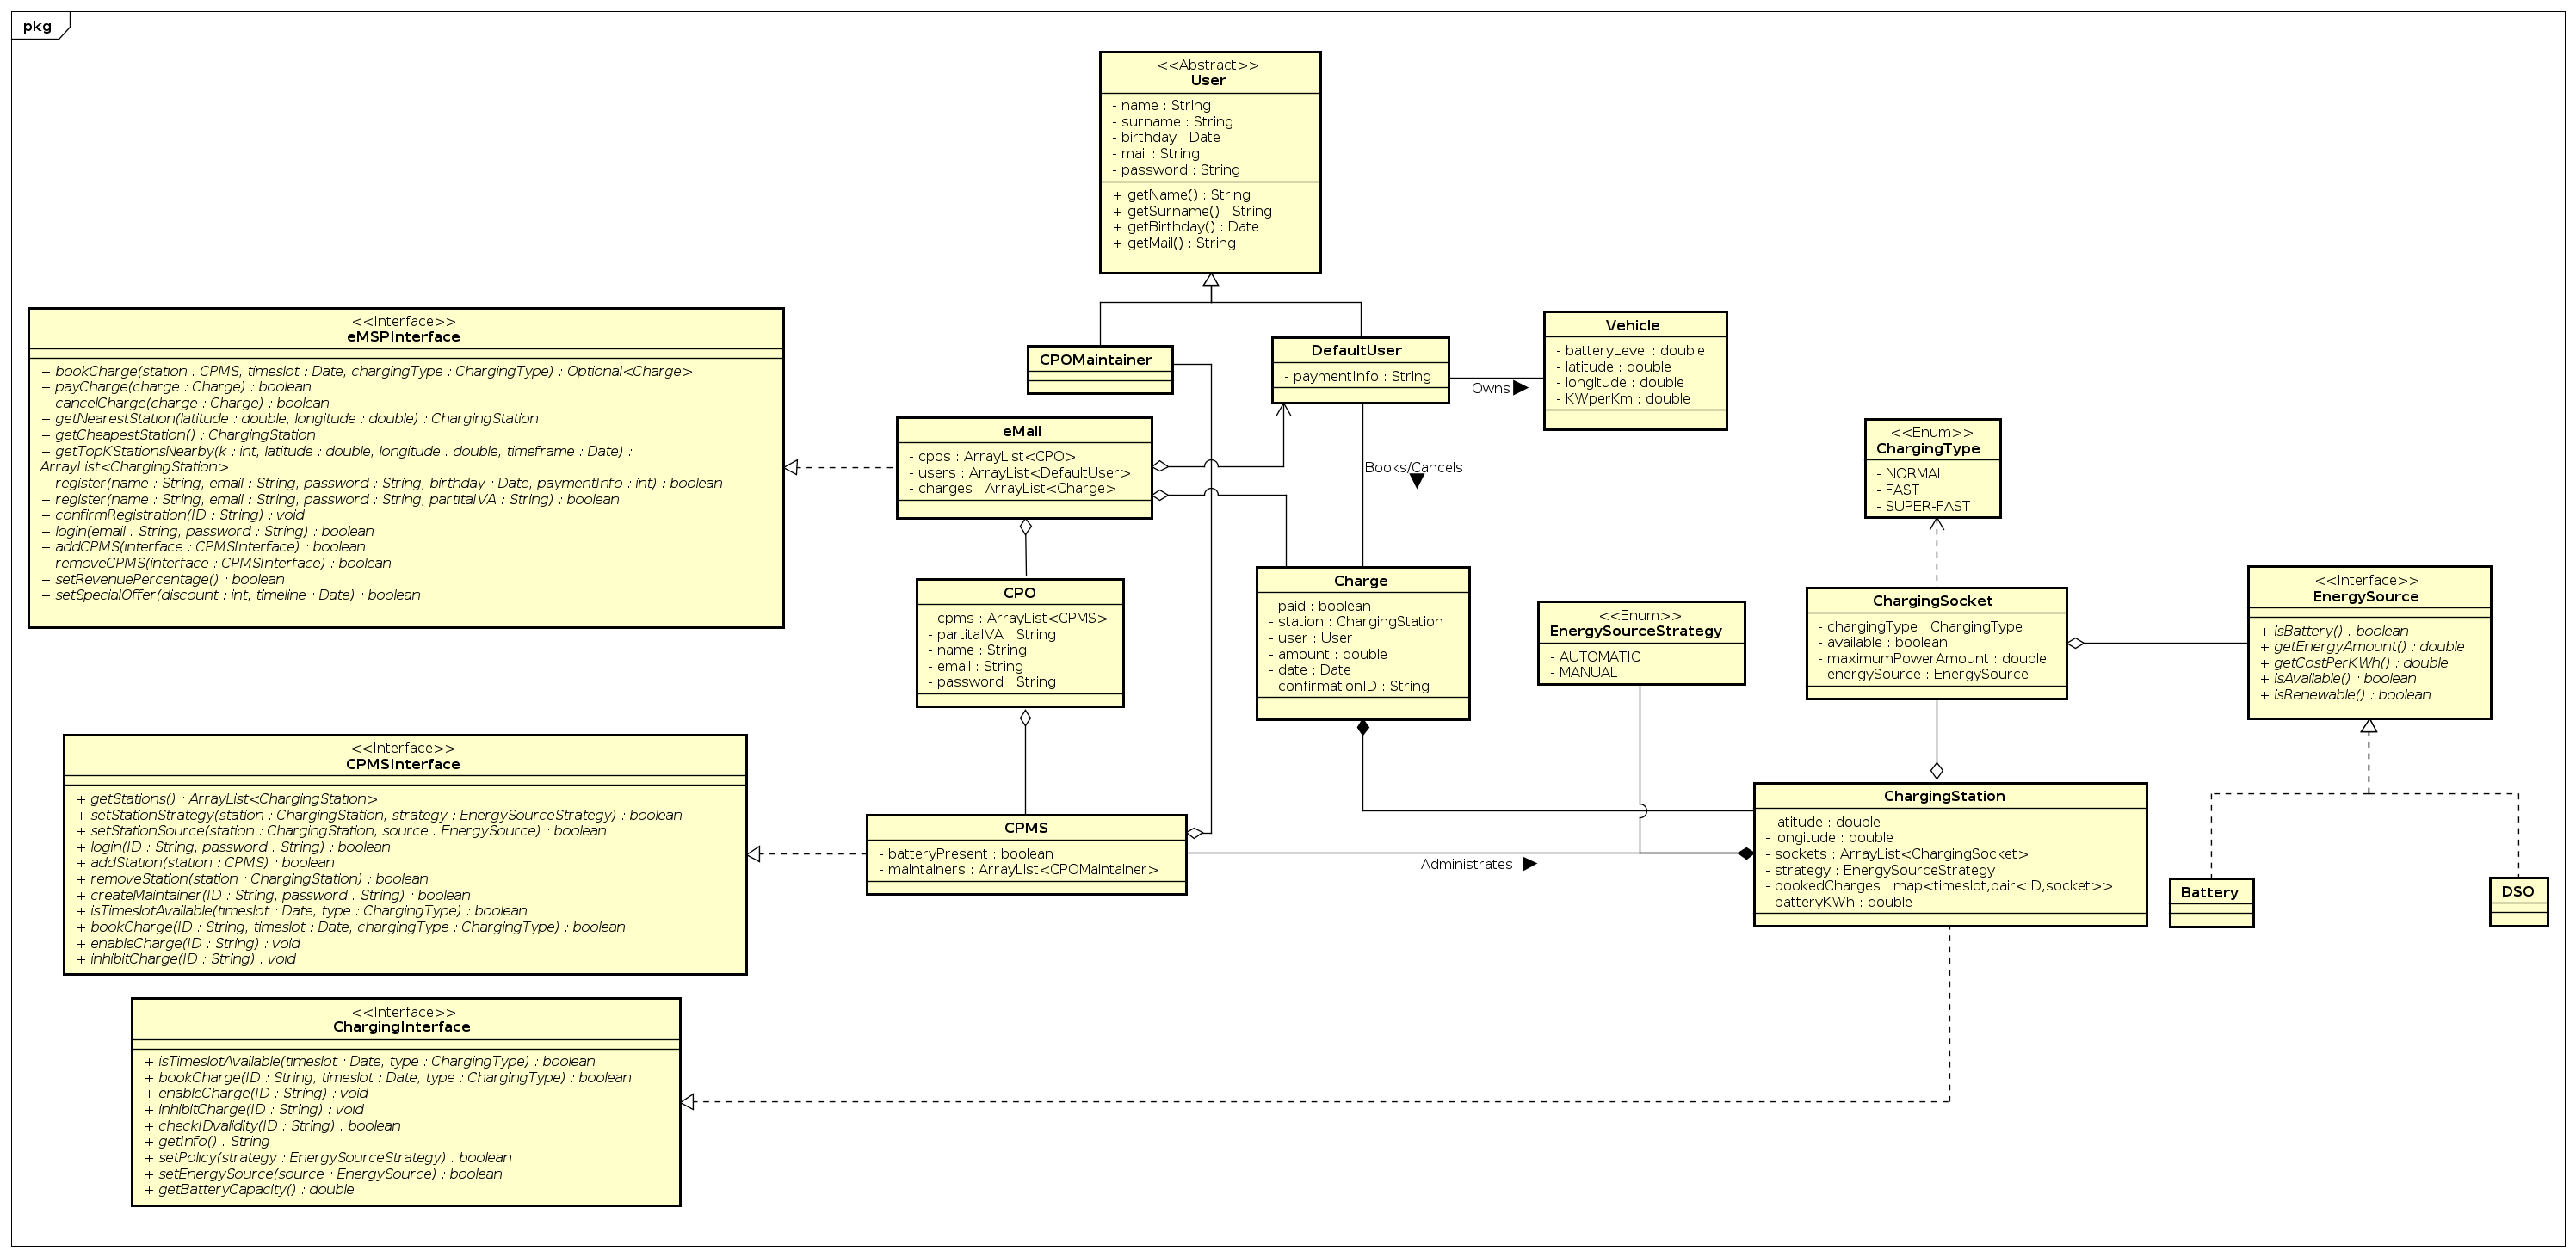
\includegraphics[keepaspectratio, width=16cm]{UML.png}
        \caption{Class diagram}
        \label{fig:UML}
    \end{center}
\end{figure}
In the class diagram illustrated in \autoref{fig:UML} a model (not functional) view of the system is represented. The \ac{eMall} and \ac{CPMS} interfaces show what the two systems are expected to implement, whereas for the ChargingInterface it is assumed an already existing implementation.

\subsubsection{Component diagrams}
\begin{figure}[!h]
    \begin{center}
        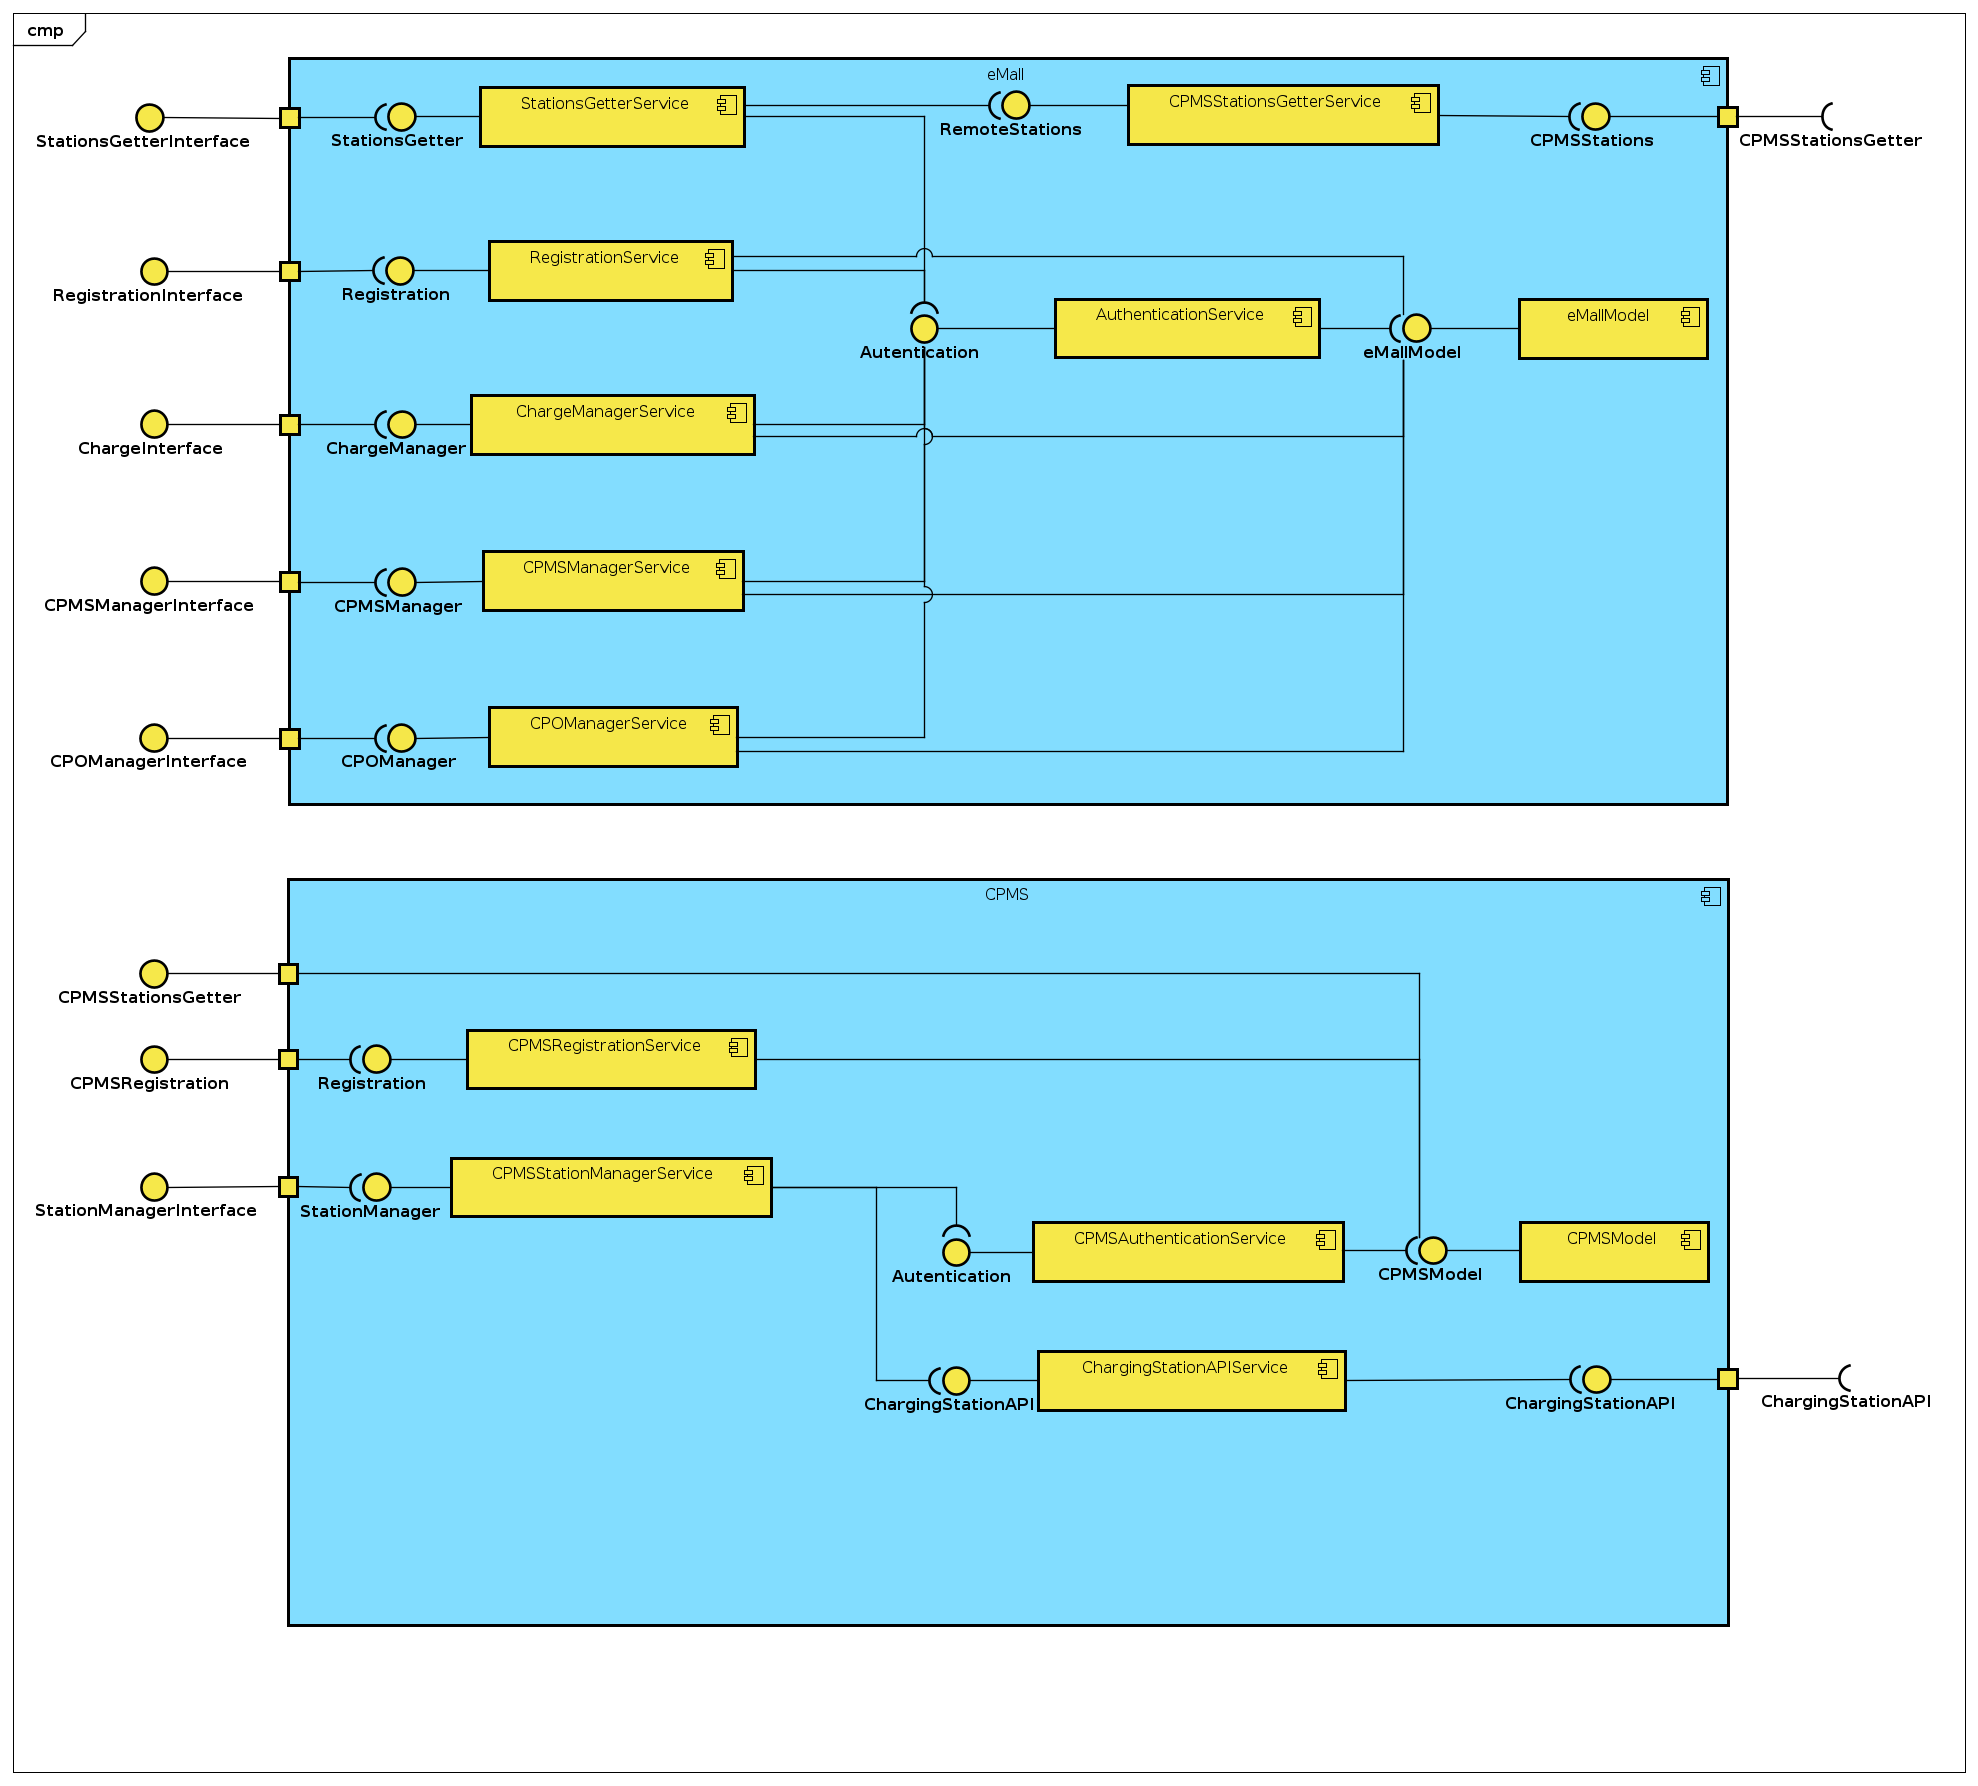
\includegraphics[keepaspectratio, width=16cm]{Component/Component.png}
        \caption{eMall component diagram}
        \label{fig:eMSP-component}
    \end{center}
\end{figure}
\clearpage
\todo[inline]{Inserire come mai ci sono interfacce di mezzo (PaymentAPI) e non direttamente il collegamento con le interfacce esterne: perchè convertono le interfacce.}
The two systems implement different interfaces and represent the \textit{Controller} and \textit{Model} parts of the \ac{MVC} pattern.

\paragraph{\textbf{\ac{eMall}}}
The main components for the \ac{eMall} system are:
\begin{itemize}
    \item \textbf{StationsComponent}: It is the component responsible for handling all the stations research requests (like \textit{getNearestStations}, \textit{getCheapestStation}, \textit{getTopKStationsNearby});
    \item \textbf{RegistrationComponent}: It is the component responsible for handling the registration details along with the parameters checking during the registration phase;
    \item \textbf{ChargeManagerComponent}: It is the component responsible for handling all the charge booking/payment/cancellation processes. \\ It interfaces with the payment \ac{API} and with the charging station \ac{API};
    \item \textbf{\ac{CPMS}ManagerComponent}: It is the component responsible for handling the \ac{CPMS} operations from the \acp{CPO} users;
    \item \textbf{\ac{CPO}ManagerComponent}: It is the component responsible for handling the \acp{CPO} requests (like \textit{SetRevenuePercentage} and \textit{setSpecialOffer});
    \item \textbf{\ac{CPMS} \ac{API}}: It is the component responsible for interfacing the \ac{eMall} with the CPMS interfaces;
    \item \textbf{AuthenticationComponent}: It is the component responsible for authorizing every operation over the model component. At this level it is implemented part of the controller (of the \ac{MVC} pattern) to check that operation is legit for the account type;
    \item \textbf{Payment \ac{API}}: It is a component that interfaces the \ac{eMall} system with the external payment \acp{API};
    \item \textbf{\ac{eMall}Model}: It is the core component. It stores all the \ac{eMall} data and interfaces them with the other system components.
\end{itemize}
There are some apparently similar components with some slight differences:
\begin{itemize}
    \item The \ac{CPO} manager component is conceptually different from the \ac{CPMS} manager component because the CPMS manager Component alters the stations collection of the model according to the interface with the inserted \ac{CPMS};
\end{itemize}
\paragraph{\textbf{\ac{CPMS}}}
The main components for the \ac{CPMS} system are:
\begin{itemize}
    \item \textbf{\ac{CPMS}RegistrationComponent}:
    \item \textbf{\ac{CPMS}StationManagerComponent}:
    \item \textbf{\ac{CPMS}ChargeManagerComponent}:
    \item \textbf{\ac{CPMS}AuthenticationComponent}:
    \item \textbf{\ac{CPMS}ChargingStation \ac{API}}:
    \item \textbf{\ac{CPMS}Model}:
\end{itemize}

\subsection{Deployment view}
\todo[inline]{Menzionare Costi}

\subsubsection{\ac{eMSP}}
\begin{figure}[!h]
    \begin{center}
        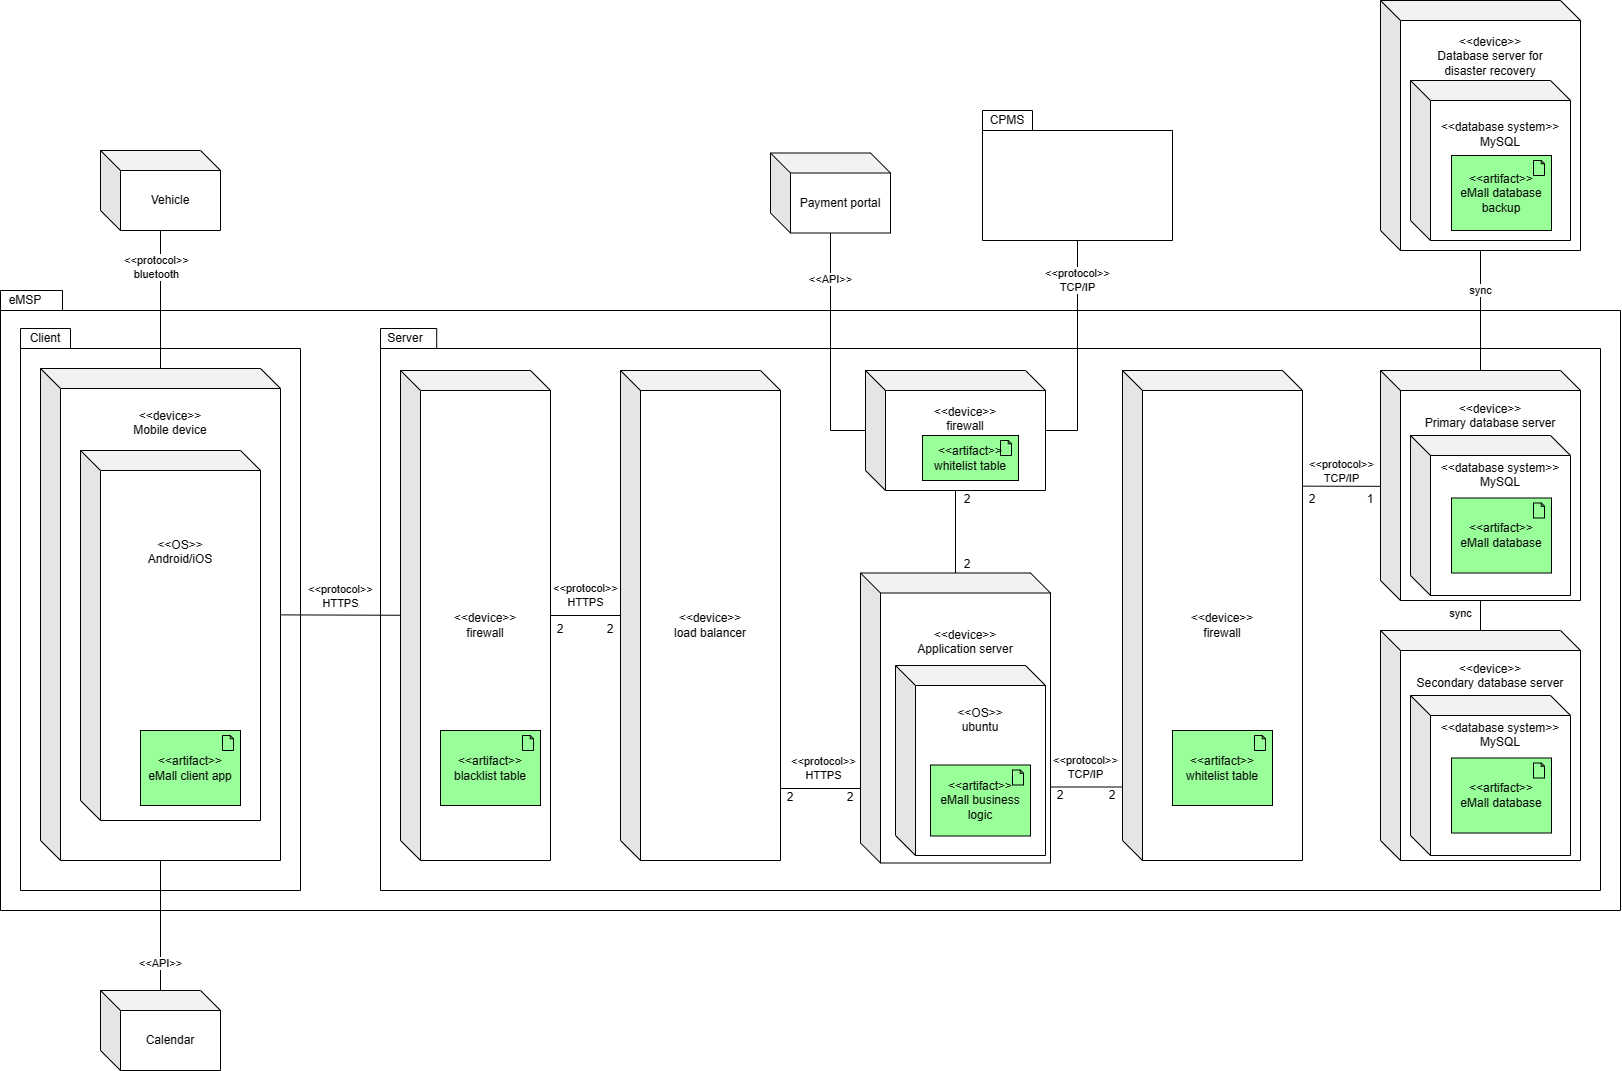
\includegraphics[keepaspectratio, width=0.9\textwidth]{Graphics/DD-eMSP-deployment.drawio.png}
        \caption{eMall deployment view diagram}
        \label{fig:eMSP-deployment}
    \end{center}
\end{figure}

The system has been designed in order to avoid \acp{SPOF}, in order to be used by an high availability service, and to support security policies. So the components of the system are:
\begin{itemize}
    \item Mobile device: It is the device used by users or \acp{CPO} to interact with the \ac{eMall} system. It is provided with internet connection, bluetooth peripheral and the \ac{eMall} client application installed. This application must be available for both Android and iOS mobile operative systems in order to be available by the most part of the people.
    Uses \ac{HTTPS} to communicate with the server or the calendar in order to exploit all the security layers implemented by it, following, in this way, also the \ac{GDPR} law. Uses bluetooth (or whatever protocol used by vehicles to create a PAN) in order to retrieve vehicle infos. 
    \item Application server: server that receives all the requests from the clients and hosts the business logic. There are two redundant application servers in order to increase reliability and availability while also avoiding down-times while maintaining the \ac{eMall} service.
    \item Load balancer: balances the load of the requests on the different application servers and handles the case if one application server is down. This system provides failover as described in \cite{ref:redundant-load-balancers}.
    \item Firewall: Each firewall in the server is used to isolate different zones. A first firewall interfaces the external world to the load balancer in order to filter dangerous requests.
    Blacklist rule table is implemented for the impossibility to implement an allowlist. For the firewall that interfaces the application server to the database an allowlist rule table is implemented because the only traffic permitted to the database is the one coming from the application servers. This system provides failover as described in \cite{ref:redundant-firewalls}.
    \item Database system: A redundant database system is implemented where the secondary database should always be synced with the primary in order to be ready for substituting the primary one in case of failure as described in \cite{ref:redundant-databases}. Also a disaster recovery database is necessary since data is of primary importance in this application. MySQL DBMS has been chosen because it is one of the most used relational DBMS \cite{ref:most-popular-RDBMS}.
\end{itemize}
\todo[inline]{Protocol used: (application server - CPMS) and (user device - server)}
\subsubsection{\ac{CPMS}}
\begin{figure}[!h]
    \begin{center}
        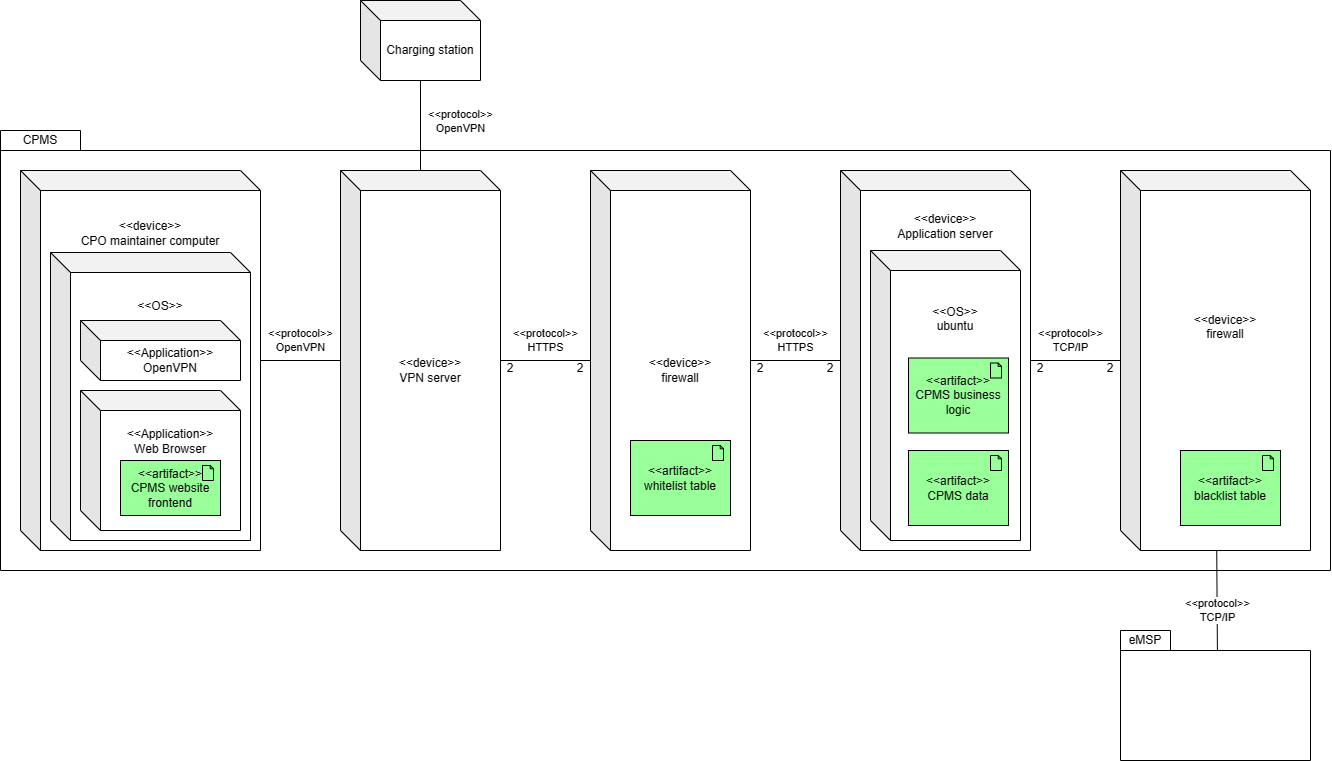
\includegraphics[keepaspectratio, width=0.9\textwidth]{Graphics/DD-CPMS-deployment.drawio.png}
        \caption{CPMS deployment view diagram}
        \label{fig:CPMS-deployment}
    \end{center}
\end{figure}

For the \ac{CPMS} the concept is to keep all the communication as in a private network, implementing a \ac{VPN} for the remote nodes (i.e. the \ac{CPO} maintainer personal computer and the charging stations) so that only people in that \ac{VPN} have the ability to perform maintainer's actions. The only point where remote connections happen is from \acp{eMSP}. Another important factor is the redundancy of the systems, in order to avoid \acp{SPOF}.
\begin{itemize}
    \item \ac{CPO} maintainer computer: This device is connected through a \ac{VPN} to a \ac{VPN} server. It runs the management software for the \ac{CPMS} the maintainer wants to administrate on top of an Ubuntu operative system, the most used linux distro according to \cite{ref:most-popular-linux-distro}. 
    In our architecture this is the thin client, in fact the \ac{CPMS} management software just handles the view of the information retrieved and sends commands to the application server. All the business logic will be contained in the application server.
    \item \ac{VPN} server: It permits the \ac{CPO} maintainer computers, the charging stations and the application server to share the same network in order to simplify the communication among the components. The OpenVPN protocol \cite{ref:openvpn-site} has been chosen because it is an open source project and is very widely used in many different applications. This system provides failover as described in \cite{ref:redundant-VPN-servers}.
    \item Application server: This is the component that handles all the commands issued to the system and redirects them to the charging stations if needed. It is surrounded by firewalls so that we can enforce security policies, such as blocking particular public IPs or allow only some internal IPs corresponding to the charging stations or the \ac{CPO} maintainer computers. This system is redundant in order to assure the continuity of availability during maintenance.
    \item Firewalls:
\end{itemize}
\todo[inline]{Added <<API>>}
\todo[inline]{Protocol used: (eMSP - application server)}
\clearpage

\subsection{Runtime view}
\subsection{Component interfaces}
\subsection{Selected architectural styles and patterns}
\subsection{Other design decisions}
\clearpage